\documentclass[12pt]{report}

\usepackage{polyglossia}
  \setmainlanguage{spanish}
\usepackage{fontspec}
  \setmonofont[Scale=.9]{Ubuntu Mono}
\usepackage[libertine, mono=false]{libertine}
\usepackage[libertine]{newtxmath}
\usepackage{microtype}
\usepackage{amsmath}
\usepackage[explicit]{titlesec}
  % Estilo de los titulos de capitulos:
  \newlength\chapnumb
  \setlength\chapnumb{4cm}
  \newcommand{\chaptertitlefont}{\normalfont\sffamily\Huge}
  \titleformat{\chapter}[block]
  {\normalfont\sffamily}{}{0pt}
  {\parbox[b]{\chapnumb}{%
     \fontsize{120}{110}\selectfont\thechapter}%
    \parbox[b]{\dimexpr\textwidth-\chapnumb\relax}{%
      \raggedleft%
      \hfill{\chaptertitlefont#1}\\
      \rule{\dimexpr\textwidth-\chapnumb\relax}{0.4pt}}}
  \titleformat{name=\chapter,numberless}[block]
  {\normalfont\sffamily}{}{0pt}
  {\parbox[b]{\chapnumb}{%
     \mbox{}}%
    \parbox[b]{\dimexpr\textwidth-\chapnumb\relax}{%
      \raggedleft%
      \hfill{\chaptertitlefont#1}\\
      \rule{\dimexpr\textwidth-\chapnumb\relax}{0.4pt}}}
\usepackage{geometry}
\usepackage{parskip}
\usepackage{tcolorbox}
\usepackage{tocloft}
  \setlength{\cftsubsecindent}{5em}
\usepackage{mathtools}
  \newtagform{brackets}{[}{]}
  \usetagform{brackets}
\usepackage{subcaption}
\usepackage{tikz}
  \usetikzlibrary{arrows}
\usepackage{pgfplots}
  \pgfplotsset{compat=1.12}
  \makeatletter
    \pgfdeclareplotmark{dot}
      {%
        \fill circle [x radius=0.04, y radius=0.16];
      }%
  \makeatother
\usepackage{booktabs}
\usepackage{makeidx}
  \makeindex
\usepackage[backend=bibtex,style=authoryear,citestyle=authoryear,doi=false,isbn=false,url=false]{biblatex}
  \addbibresource{NER-bib.bib}
\usepackage[hidelinks,spanish]{hyperref}

%pgfplot función normal
\pgfmathdeclarefunction{gauss}{2}{%
  \pgfmathparse{1/(#2*sqrt(2*pi))*exp(-((x-#1)^2)/(2*#2^2))}%
}

\newcommand*{\eng}[1]{\textsl{#1}}
\newcommand*{\paq}[1]{\textbf{#1}\index{#1@\textbf{#1}}}
\newcommand*{\kw}[1]{\textbf{#1}\index{#1}}

\newcommand{\Var}{\operatorname{Var}}
\newcommand{\Cov}{\operatorname{Cov}}
\newcommand{\E}{\operatorname{E}}
\newcommand{\sd}{\operatorname{sd}}
\newcommand{\se}{\operatorname{se}}

% Eliminar numeración en títulos menores que secciones
\setcounter{secnumdepth}{1}

% Color box para R
% new tcolorbox environment
% #1: tcolorbox options
% #2: color
% #3: box title
\newtcolorbox{Rbox}[1][]
{
  title = El c\'odigo R,
  fonttitle=\sffamily\bfseries,
  colbacktitle=black!35!white,
  colframe=black!35!white,
  fontupper=\sffamily,
  colupper=black!80!white
  #1,
}

% Knitr setup



\title{Notas de Econometría en R}
%\thanks{Estas notas son un intento de condensar lo justo y necesario para poder seguir un curso de econometría con R.Luego de recopilar material de muchas clases y ayudantías de econometría, en general pensadas para ser aplicadas en Stata, decidí que podía intentar hacer estas clases en R y usar esta guía como material de apoyo.Mi prioridad fue ser breve y conciso, por lo que estas notas no son un buen comienzo para aprender R (o econometría); son un complemento.Si hay algún error o quieres hacer algún comentario, mi correo es \texttt{acarril@fen.uchile.cl}.}
\author{Alvaro Carril}
\date{Borrador, \today \\
  \includegraphics[width=\textwidth]{figs/scatterplot3d_portada}
}


\begin{document}

\maketitle
\tableofcontents

\clearpage

% Introducción, prefacio:



\chapter{Introducción}

En las últimas décadas la economía ha ido adoptando a los computadores para realizar econometría aplicada.
Sin embargo, la manera en que se enseña econometría sigue siendo eminentemente teórica.
La gran mayoría de los textos de econometría deriva los modelos como ejercicios de álgebra lineal, y más tarde (o nunca) intentan conectar esto con el trabajo aplicado, usando ejemplos específicos y pequeños extractos de código (si es que hay algo de código).
Este libro intenta dar la vuelta a este paradigma, apoyándose en R desde un comienzo y en forma continua durante el desarrollo de las ideas.

%A mi parecer, existen actualmente dos maneras de abordar la enseñanza de econometría. La primera es la clásica, o \emph{matemática}: derivando los modelos desde como ejercicios de álgebra lineal, y en general priorizando aspectos técnicos por sobre los conceptuales o aplicados. Vemos esto en libros que discuten en extensión los supuestos detrás de las formas funcionales o supuestos de distribución, pero que dedican pocas palabras a técnicas aplicadas como métodos de regresión discontinua.

%Por otro lado hay quienes, de la mano con el crecimiento de la economía aplicada, abogan por una enseñanza aplicada de econometría, con énfasis en técnicas de 

\section{¿Qué es R?}

R es un ambiente de software y un lenguaje de programación interpretado para manipular datos, hacer análisis estadístico y visualizar datos. Es una implementación de S, un lenguaje de programación matemático orientado a objetos más antiguo. Es software libre y de código abierto, constantemente desarrollado y ampliado por colaboradores de múltiples disciplinas.

R es mucho más flexible que la mayoría de los paquetes estadísticos normalmente usados por economistas. Es un lenguaje de programación completamente desarrollado, no sólo un programa con tests y métodos pre-programados.

\section{Obtener R}

La instalación base de R puede obtenerse directamente de \url{https://cloud.r-project.org/}. Una vez instalado puedes usar RGui para interactuar con R. Sin embargo, esta opción no es demasiado sexy:

\begin{center}
\vspace{\baselineskip}
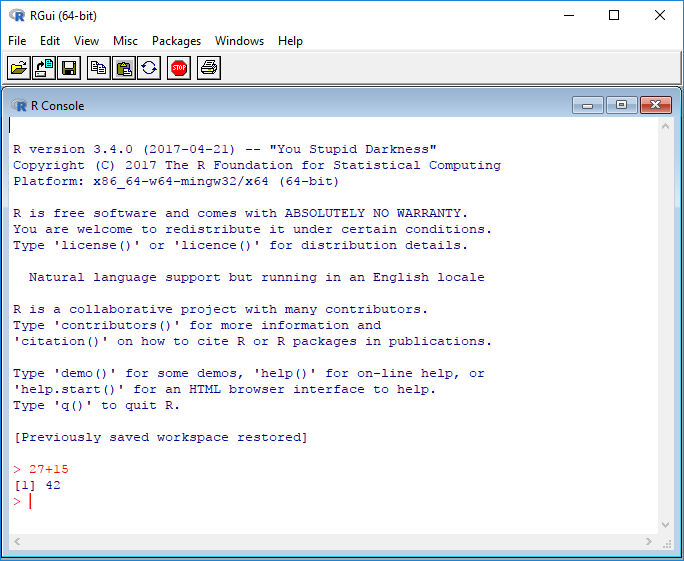
\includegraphics[width=.66\linewidth]{sss/rgui-win-42}
\vspace{\baselineskip}
\end{center}

Mi recomendación es usar RStudio, un IDE (\eng{integrated development environment}) que nos ayudará a trabajar mucho más cómodamente con R. RStudio incluye una consola, un editor de código con resaltado de sintaxis, explorador de objetos y una larga lista de cosas que puede que no entiendas aún, pero que seguro harán tu vida más fácil. Con toda seguridad se \emph{ve} mejor que RGui. Puedes descargar RStudio de \url{https://www.rstudio.com/}, y también es gratis (asegúrate de haber instalado R antes de instalar RStudio).

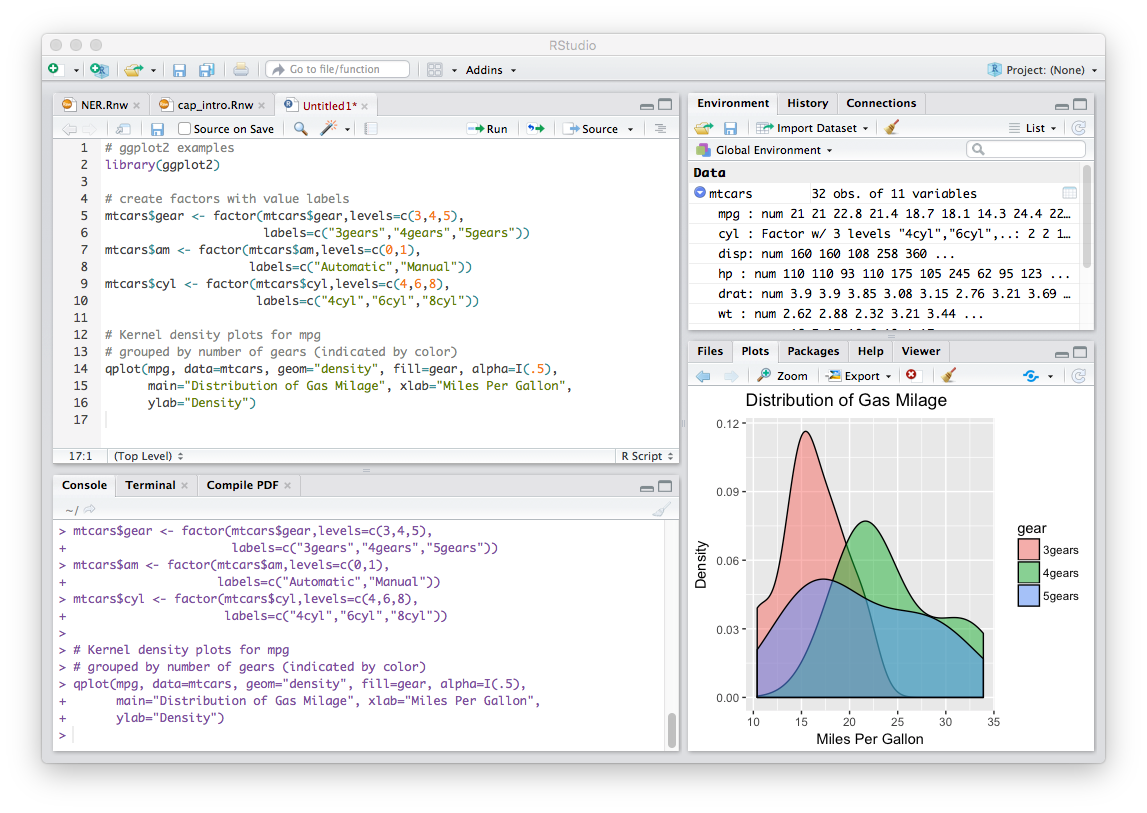
\includegraphics[width=\linewidth]{sss/rstudio-mac}

\subsection{Usar R interactivamente y a través de scripts}

\subsection{Trabajando con datos}

\subsubsection{Objetos y asignaciones}

R es un lenguaje interpretado, lo que significa que ejecuta nuestras instrucciones directamente, sin compilar un programa previo. Podemos usar R interactivamente a través de la consola:
\begin{knitrout}
\definecolor{shadecolor}{rgb}{0.969, 0.969, 0.969}\color{fgcolor}\begin{kframe}
\begin{alltt}
\hlnum{1}\hlopt{+}\hlnum{2}
\end{alltt}
\begin{verbatim}
## [1] 3
\end{verbatim}
\end{kframe}
\end{knitrout}

La mayoría de las operaciones y funciones en R no guardan el resultado de su ejecución. Por ejemplo, el resultado anterior (\verb|3|) es calculado pero no puede ser reutilizado sin volverse a calcular. Para lograr esto tenemos que asignar el resultado de la operación a un objeto:
\begin{knitrout}
\definecolor{shadecolor}{rgb}{0.969, 0.969, 0.969}\color{fgcolor}\begin{kframe}
\begin{alltt}
\hlstd{x} \hlkwb{<-} \hlnum{1}\hlopt{+}\hlnum{2}
\end{alltt}
\end{kframe}
\end{knitrout}

\section{R base vs. tidyverse}
\label{sec:rbase_tidyverse}

Una de las críticas más comunes que se hace a R es que hay muchas (¿demasiadas?) maneras de lograr un mismo resultado. Por ejemplo, R base tiene un sistema propio para crear gráficos, pero también existe \paq{ggplot2} para lograr el mismo objetivo.
Esta multiplicidad de métodos puede hacer que R sea más difícil de aprender que lo necesario.

R es un lenguaje antiguo, y muchas de sus funcionalidades básicas ---lo que llamamos \kw{R base}--- operan bajo paradigmas anticuados. Uno de los más grandes aportes a la programación en R del útltimo tiempo fue realizado por Hadley Wickham, principal autor del \paq{tidyverse}. Este es un conjunto de paquetes que modernizan cómo usamos R para manipular datos, y están diseñados para trabajar bien entre ellos.

En un artículo para R-bloggers\footnote{\url{https://www.r-bloggers.com/teach-the-tidyverse-to-beginners/}}, David Robinson resume los dos principales ``curriculums'' de aprendizaje de R:
\begin{itemize}
\item \textbf{R base primero}: enseñar elementos de sintaxis como \verb|$| y \verb|[[]]|, loops, condicionales, tipos de datos y funciones base como \verb|tapply()|. Este enfoque no se concentra en un sólo marco de datos.
\item \textbf{tidyverse primero}: comenzar usando \paq{dplyr} para manipular marcos de datos y \paq{ggplot2} para crear gráficos. Luego introducir rápidamente el uso de \paq{tidyr} y \paq{purrr}. Usar el operador \verb|%>%| casi inmediatamente, pero dejar el uso de \verb|$| y \verb|[[]]| para más adelante. Este enfoque se concentra en un sólo marco de datos.
\end{itemize}

Mi opinión (y la de muchos otros) es que aprender a usar las herramientas del \paq{tidyverse} es más fácil y más productivo. La filosofía detrás del \paq{tidyverse} es similar a la de Python: "Debería haber una ---y preferiblemente sólo una--- forma obvia de lograr algo''. Esta filosofía es buena al aprender un lenguaje de programación, ya que es más consistente y evita confusiones.
Es por esto que en este documento prefiero usar herramientas del \paq{tidyverse} cada vez que sea posible.

Por ejemplo, en R base existen al menos tres formas de crear una variable nueva a partir de otra existente.
Por otro lado, con el \paq{tidyverse} hay una sóla forma de lograr esto, que además (a mi) me parece más legible:

\begin{knitrout}
\definecolor{shadecolor}{rgb}{0.969, 0.969, 0.969}\color{fgcolor}\begin{kframe}
\begin{alltt}
\hlcom{# Agregar una variable con R base}
\hlstd{mtcars}\hlopt{$}\hlstd{libras} \hlkwb{<-} \hlstd{mt}\hlopt{$}\hlstd{wt} \hlopt{*} \hlnum{1000}
\hlstd{mtcars[[}\hlstr{"libras"}\hlstd{]]} \hlkwb{<-} \hlstd{mtcars[[}\hlstr{"wt"}\hlstd{]]} \hlopt{/} \hlnum{1000}
\hlstd{mtcars[,} \hlstr{"libras"}\hlstd{]} \hlkwb{<-} \hlstd{mtcars[,} \hlstr{"wt"}\hlstd{]} \hlopt{/} \hlnum{1000}

\hlcom{# Agregar una variable con el tidyverse}
\hlstd{mtcars} \hlkwb{<-} \hlstd{mtcars} \hlopt \hlkwd{mutate}\hlstd{(}\hlkwc{libras} \hlstd{= wt} \hlopt{/} \hlnum{1000}\hlstd{)}
\end{alltt}
\end{kframe}
\end{knitrout}

Sin embargo, también hay elementos de R base que son importantes de aprender; de hecho, muchas cosas en R no son posibles sin ellos. Iremos introduciendo estos elementos a medida que nos sean útil para el tema en cuestión.

\section{Detalles técnicos}

Este documento fue compilado usando R 

% Regresión lineal bivariada:


